% v3 manuscript, anonymised for double-blind review (the title page with author details is title_page.tex).
% Generated by paper/v3/build.py from the verified runs accoding-learner-v3 and accoding-policy-v3;
% edit this template or the section files, never the generated manuscript.tex.
\documentclass[a4paper,preprint,12pt,authoryear]{elsarticle}
\usepackage{amsmath,amssymb}
\usepackage{booktabs}
\usepackage{graphicx}
\usepackage[table]{xcolor}
\usepackage[hidelinks,hypertexnames=false]{hyperref}
\usepackage[capitalise,noabbrev]{cleveref}
\usepackage{microtype}
\usepackage{float}
\setlength{\emergencystretch}{3em}
\pdfpagewidth=\paperwidth \pdfpageheight=\paperheight % A4 media box (XeTeX ignores the class paper option)
\newtheorem{proposition}{Proposition}
\crefname{proposition}{Proposition}{Propositions}
\renewcommand{\appendixname}{Appendix} % elsarticle already inserts a tie before the letter
\makeatletter
% Appendix floats numbered per appendix (Table A.1, Fig. A.1), as the journal's guide requires
\g@addto@macro\appendix{\@addtoreset{table}{section}\@addtoreset{figure}{section}}
\makeatother
\journal{Comput. Educ.: Artif. Intell.}

\begin{document}
\begin{frontmatter}

\title{Do knowledge-tracing simulators reward learning? A negative-control audit of reinforcement-learning exercise recommendation for programming}

\begin{abstract}
Reinforcement-learning (RL) agents that choose programming exercises are commonly trained and evaluated inside a knowledge-tracing (KT) model fitted to learner logs, which also measures their benefit. We audited this practice on 562,912 first attempts by 4,634 learners of a C-programming online judge, none of whom were used before the study protocols were locked. Six learner models, including deep knowledge tracing (DKT), forecast held-out learners equally well (AUC 0.775--0.776), and an entropy-based identification tree gave interpretable diagnoses. DQN and PPO agents trained with a DKT reward exceeded random selection by 13.2 and 27.2 percentage points of expected post-test success in their training simulator, but by at most 0.35 points in independently fitted worlds with explicit latent learning. In a negative-control world where learning is impossible, the DKT tracker still reported gains of 12.8 and 25.7 points for these agents, and across 14 policies in-simulator gain was almost perfectly rank-correlated with this phantom gain (Spearman 0.960). We show that a policy's expected gain inside a KT simulator equals the model's accumulated self-predicted change (drift), which is zero for coherent models without learning; DKT's drift was 16 times more dispersed across problems than that of an additive factor model and was poorly reproduced by a re-seeded DKT. Agents trained in a world with explicit practice-driven learning transferred best across latent worlds of that family, but not to neural worlds. We recommend negative-control worlds, drift reporting and independently fitted worlds as standard checks for simulator-based evaluation of adaptive recommenders.
\end{abstract}

\begin{keyword}
knowledge tracing \sep reinforcement learning \sep exercise recommendation \sep programming education \sep simulation-based evaluation \sep negative control
\end{keyword}

\end{frontmatter}

\section{Introduction}\label{sec:intro}

Programming courses assign many small exercises, and learners progress at very different speeds. An exercise that is too difficult discourages a learner; one that is too easy teaches little. Adaptive exercise recommendation addresses this by estimating each learner's state from past attempts and choosing the next exercise accordingly, an idea often motivated by the zone of proximal development \citep{vygotsky1978mind} and with a long tradition in adaptive educational systems for programming \citep{brusilovsky2007user,hsiao2010guiding}. A now common recipe combines a knowledge-tracing (KT) model, which forecasts a learner's success on each exercise from their history, with a reinforcement-learning (RL) agent that treats the choice of exercise as a sequential decision problem: the learner model's state is the agent's state, recommending an exercise is an action, and an increase in the model's predicted knowledge is the reward \citep{huang2019dre,liu2019cseal,ai2019cdkt,chen2023src,li2023gehrl,ozyurt2025exrec}. Because trials with learners are expensive, such agents are often trained \emph{and evaluated} inside a fitted learner model, and the resulting gain in predicted knowledge is reported as the benefit of the policy \citep{cheng2026unier}.

This evaluation is only as good as the simulator's account of how practice changes success on other exercises. KT models are fitted and validated on next-step forecasts of the sequences that learners actually followed. A policy, however, creates new sequences, and the simulator must extrapolate what these sequences would do. Two models can forecast observed data equally well and still disagree about such counterfactuals \citep{breiman2001two,damour2022underspecification}. For instructional decisions this was noticed early: individualised and population knowledge-tracing parameters imply very different amounts of practice \citep{lee2012individualizing}, and student models with similar predictive accuracy can recommend substantially different amounts of practice \citep{rollinson2015predictive}. The robust evaluation matrix therefore evaluates candidate policies under several student models \citep{doroudi2017rem}, and a review of RL for instructional sequencing found that policies derived from purely data-driven models often failed to outperform reasonable baselines when tested with students \citep{doroudi2019reward}. In reinforcement learning more generally, an optimiser trained against a learned model or a learned reward exploits that model's errors \citep{kurutach2018metrpo,janner2019trust,gao2023scaling}. Modern KT--RL pipelines combine both risks---the learned model is at once the environment, the reward and the yardstick---yet it is rarely quantified how much of a reported gain reflects learning that the simulator encodes and how much reflects the simulator's idiosyncrasies.

We study this question for introductory programming, using 1,291,558 judged C/C++ submissions by 4,634 learners of the ACcoding online judge \citep{chen2024accoding}. We fit six learner models of equal predictive accuracy, including deep knowledge tracing (DKT) as the deployed tracker and an entropy-based identification tree for interpretable diagnosis; train Double DQN and PPO recommenders in three kinds of training worlds; and evaluate every policy in nine worlds that differ in the learners they were fitted to and in how learning is represented. Two instruments make the evaluation diagnostic. A \emph{negative-control} world without any learning, in which the true gain of every policy is exactly zero, exposes spurious gains directly. An exact \emph{decomposition} of a tracker's reported gain into the model's own expected forecast change (\emph{drift}) and evidence \emph{surprise} shows where such gains come from. We prove that drift vanishes for coherent Bayesian models without learning and that, inside its own simulator, the expected gain of any policy equals the drift it accumulates; in-simulator evaluation therefore rewards a policy for choosing problems that the model \emph{expects} to raise its own forecast.

We address four research questions. RQ1: How well do cognitive-state models forecast first-attempt success of unseen programming learners, and do they differ? RQ2: How large are the gains of RL recommenders in the KT simulator they are trained in? RQ3: Do these gains survive independently fitted worlds, and how large are the gains a tracker reports when no learning is possible? RQ4: What produces the discrepancy, and which policies remain robust? All protocols, including four hypotheses, were locked on a development cohort before the evaluation population was loaded.

Our contributions are: (1) an end-to-end, reproducible pipeline for adaptive programming exercise recommendation on real data, from learner models to trained DQN and PPO agents and an interactive application, with pre-registered hypotheses tested on a population never used before; (2) evidence that, although six learner models forecast equally well, the in-simulator gains of KT-reward agents shrink to near zero in independently fitted worlds with latent learning and are almost perfectly rank-correlated with the gains the tracker reports in a world where no learning occurs; (3) the drift decomposition and two propositions that explain these gains as the tracker's accumulated self-predicted change rather than learning, a model-internal diagnostic that needs no additional data; and (4) exploratory evidence that agents trained in a world with explicit learning structure transfer best across latent worlds of that family---but not to neural worlds---together with inexpensive checks for simulator-based evaluation.

\Cref{sec:related} reviews related work, \cref{sec:data} describes the data and \cref{sec:methods} the models, decision problem, evaluation worlds and analysis. \Cref{sec:results} reports the results, \cref{sec:discussion} discusses their implications and limitations, and \cref{sec:conclusion} concludes.

\section{Related work}\label{sec:related}

\subsection{Learner models and knowledge tracing}

Knowledge tracing estimates a learner's evolving knowledge from response sequences. Bayesian knowledge tracing models each knowledge component as a hidden binary state \citep{corbett1994bkt}; logistic models such as the additive factor model (AFM) and performance factors analysis (PFA) combine a learner ability, item difficulty and practice counts per knowledge component \citep{cen2006lfa,pavlik2009pfa,pelanek2017learner}, in the sense of knowledge components described by \citet{koedinger2012kli}. Recurrent and attention-based models, starting with DKT \citep{piech2015dkt} and continuing with SAKT and AKT \citep{pandey2019sakt,ghosh2020akt}, learn the dynamics from data \citep[see][for a survey]{abdelrahman2023survey}. Several comparisons found that well-specified logistic models match or approach deep models in forecasting accuracy \citep{khajah2016deep,wilson2016basics,gervet2020deep}. DKT's step-to-step predictions can also move in implausible directions, for instance lowering the predicted mastery of a skill after a correct answer \citep{yeung2018dktplus}, which has motivated consistency and monotonicity constraints \citep{zhang2023cmkt}. For programming, KT has been extended with code features \citep{shi2022codedkt}, and adaptive navigation support has long guided learners to programming problems of suitable difficulty \citep{hsiao2010guiding,brusilovsky2007user}. Evaluation of learner models is nonetheless dominated by held-out predictive accuracy, although frameworks for evaluating them by their consequences for tutoring decisions have been proposed \citep{gonzalezbrenes2015leopard,huang2015multifaceted}.

\subsection{Reinforcement learning for instructional sequencing and exercise recommendation}

Instructional sequencing with RL has a long history. Policies induced from data have been tested with students in tutoring systems \citep{chi2011umuai,shen2018jedm,zhou2022hrl}, in online courses \citep{bassen2020chi} and in a narrative mathematics tutor \citep{ruan2024rltutor}; related work has used POMDP planning \citep{rafferty2016pomdp}, multi-armed bandits \citep{clement2015bandits} and approximately optimal teaching models \citep{whitehill2018teaching}. Reviews conclude that successes are real but uneven: \citet{doroudi2019reward} found that policies derived from data-driven student models often failed to outperform reasonable baselines when tested with students and that success was more likely when policies were grounded in theory-driven models, and more recent overviews point to methodological issues and to the need for larger evaluations with actual learners \citep{singla2021rleducation,riedmann2025rlreview}. In parallel, the recommender-systems literature has built deep RL recommenders of exercises and learning paths that rely on a fitted learner model---usually a KT model---for the state, the reward or the measure of learning: multi-objective exercise recommendation \citep{huang2019dre}, cognitive-structure-aware learning paths \citep{liu2019cseal}, concept-aware DKT recommendation \citep{ai2019cdkt}, set-to-sequence and hierarchical path planners \citep{chen2023src,li2023gehrl}, knowledge-state distillation \citep{li2024pksd} and ExRec, which defines rewards and task scores through calibrated KT states \citep{ozyurt2025exrec}. The UniER benchmark unifies item- and path-level recommenders under a KT-derived weighted cognitive gain \citep{cheng2026unier}, and deep RL learning-path systems also appear in this journal \citep{ruan2025adaptive}. These works advance representation and optimisation; our question is how much of a KT-measured gain survives when the world that generates outcomes is not the model that measures them.

\subsection{From predictive accuracy to instructional decisions}

That forecasting accuracy does not settle instructional decisions is a recurring finding. For a substantial share of students, population knowledge-tracing parameters implied about twice as much practice as individually fitted parameters \citep{lee2012individualizing}; student models of similar predictive accuracy can imply substantially different amounts of practice \citep{rollinson2015predictive}; knowledge-tracing parameters can be semantically degenerate even when they fit well \citep{doroudi2017identifiability}; and misspecified models can make mastery decisions inequitable across learners \citep{doroudi2019fairer}. \citet{gonzalezbrenes2015leopard} argued for evaluating student models by the tutoring decisions they induce. The robust evaluation matrix \citep{doroudi2017rem} evaluates each candidate policy under several student models and cautions against trusting a policy that looks good only under the model used to derive it. Off-policy estimators based on importance sampling evaluate policies from logged data without a simulator \citep{mandel2014offline,thomas2016dataefficient}, but they require logged action probabilities, which self-directed practice on an online judge does not provide, so simulation remains the default for exercise recommenders. In machine learning more broadly, predictors with equivalent held-out accuracy can behave very differently downstream \citep{breiman2001two,damour2022underspecification}.

\subsection{Optimising against learned models and proxy rewards}

In model-based RL, a policy optimised in a learned dynamics model exploits the model's errors, especially where data are scarce; ensembles, short model rollouts and uncertainty penalties were introduced to limit this \citep{kurutach2018metrpo,janner2019trust,yu2020mopo,moerland2023mbrl,levine2020offline}. Optimising a proxy objective can likewise raise the proxy while the intended objective stagnates---reward hacking or gaming \citep{amodei2016concrete,skalse2022reward}---and over-optimisation of a learned reward model follows predictable scaling laws \citep{gao2023scaling}. Simulators of recommender systems inherit the biases of the logs they are fitted to \citep{huang2020keeping}, and offline evaluation is a recognised obstacle to deploying RL in the real world \citep{dulacarnold2021challenges}. KT--RL recommenders sit at the intersection of these problems because one learned model serves as dynamics, reward and evaluation metric. From epidemiology we borrow the negative control, an analysis in which the true effect is known to be absent so that any estimated effect reveals bias \citep{lipsitch2010negative,arnold2016negative}.

Our work connects these threads for programming exercise recommendation. We fit six learner models of equal predictive quality to the same real data and show how their disagreement propagates to policy rankings, and we add two instruments that the robust-evaluation literature has not used: a no-learning negative-control world, in which the true gain of every policy is exactly zero, and an exact decomposition of a tracker's reported gain into drift and surprise, with formal results that identify in-simulator gain with accumulated drift.

\section{Data}\label{sec:data}

\paragraph{Source} We use the public ACcoding dataset, version 2.0.0 \citep{chen2024accoding,sun2026accodingdata}, released by the teaching group of Beihang University for courses in C programming, data structures and algorithm analysis. The archive (SHA-256 prefix \texttt{26b5637d}) contains anonymised submissions with judge verdicts, problem metadata with a 1--10 difficulty rating assigned by educators, and 96 knowledge-point tags that the dataset article describes as defined by educators or teaching assistants. The SQL tables were parsed as text; no submitted code or SQL was executed.

\paragraph{Population and unit of analysis} Two cohorts of 1,500 learners each had been used in earlier, unpublished forecasting analyses of this archive. To keep every result reported here confirmatory, the present study uses only the 4,634 learners who were absent from both cohorts and had at least 20 distinct problems in the snapshot. One \emph{interaction} is a learner's first judged submission on a problem; the label is 1 when that submission is accepted. Unfinished (WT/JG) and judge-side or unclassified statuses (IFNR, OFNR, EFNR, OE) were removed before sequencing, and only C/C++ submissions were kept. The resulting data contain 562,912 first-encounter interactions on 3,882 problems. As an observable proxy for solving effort we record the number of submissions up to and including the first acceptance.

\paragraph{Skills} We grouped the 96 educator tags into 15 course-level skills (e.g.\ loops, arrays, strings, pointers and linked lists, recursion); problems without tags form a sixteenth group. The groups play the role of knowledge components \citep{koedinger2012kli}, but the grouping is an explicit modelling decision of the authors, released with the code, and not a validated knowledge-component model. Items carry normalised tag weights, so multi-skill problems contribute to several skills.

\paragraph{Partitions} Learners were ranked by a salted SHA-256 hash of their anonymised identifier and split into three disjoint partitions before any outcome of this population was inspected: A (1,854 learners) fits the deployed tracker and all training simulators; B (1,854 learners) fits independent evaluation worlds; T (926 learners) is used only for forecast evaluation and as starting points of evaluation episodes. Ten per cent of A and of B are inner-validation learners used for early stopping and model selection.

\section{Methods}\label{sec:methods}

\subsection{Learner models}\label{sec:learners}

Let $H_t=((j_1,y_1),\dots,(j_{t-1},y_{t-1}))$ be a learner's history of problems and first-attempt outcomes. Each model outputs $P_M(y=1\mid j,H_t)$ for any query problem $j$ and is updated after each observed outcome.

\paragraph{Logistic family with online ability} For IRT, AFM and PFA \citep[see][for an overview of this family]{pelanek2017learner},
\begin{equation}
\operatorname{logit} P(y=1\mid j,H_t,\theta) = \theta - \beta_j + \ell_M(j,H_t),
\label{eq:logistic}
\end{equation}
where $\beta_j = b_0 + b_d\,d_j + \sum_k w_{jk} b_k + u_j$ combines the released difficulty $d_j$, skill offsets and a regularised problem-specific term. The learning term is $\ell_{\mathrm{IRT}}=0$, $\ell_{\mathrm{AFM}}=\sum_k w_{jk}\gamma_k\log(1+n_k)$ with weighted practice counts $n_k$ \citep{cen2006lfa}, and $\ell_{\mathrm{PFA}}=\sum_k w_{jk}(\gamma_k\log(1+s_k)+\rho_k\log(1+f_k))$ with success and failure counts \citep{pavlik2009pfa}. Parameters are fitted by penalised maximum likelihood (Gaussian priors on $\theta$ and $u_j$). For a new learner, ability is integrated on a 101-point grid with the fitted prior and updated by Bayes' rule after every outcome, so forecasts use only the learner's own past.

\paragraph{DKT and SAKT} DKT \citep{piech2015dkt} feeds $[e_j; y e_j; y]$ to an LSTM, where $e_j$ sums a problem embedding (problems with at least ten fitting learners), a skill projection and a difficulty term; a question-conditioned decoder with a Rasch-style scalar offset, as in AKT \citep{ghosh2020akt}, outputs the next-step probability. SAKT \citep{pandey2019sakt} lets each query attend causally to the most recent 200 interactions, with a fixed per-head recency penalty on attention logits \citep{press2022alibi}; this makes chunked training and step-by-step inference identical. Hyperparameters were chosen on a development cohort only (\cref{sec:protocol}). A second DKT with a different random seed (\emph{twin}) is fitted on A with identical data and settings.

\paragraph{Entropy-based identification tree} Following the topic specification, an ID3 tree \citep{quinlan1986id3} is grown with information gain on eight interpretable history features (e.g.\ prior success on the item's skill, recent success, released difficulty, problem pass rate in A) and reduced by reduced-error pruning on inner-validation learners. Its leaves yield human-readable diagnostic rules.

\subsection{Exercise recommendation as a sequential decision problem}\label{sec:mdp}

A decision is taken after a real prefix of a learner's history. The action set is a pool of 109 problems chosen by a fixed rule from partition-A support counts only (up to 12 per fundamental skill, each attempted by at least 5\% of A learners), excluding problems already met. A disjoint post-test $\mathcal W$ of 16 problems (two per assessed skill) measures progress. The deployed \emph{tracker} is DKT fitted on A; the agent's state concatenates the tracker's predicted success on every pool problem, per-skill averages, the eligibility mask, the tracker's post-test forecast and the remaining horizon. An episode lasts ten problems. The reward operationalises the topic's objective of improving scores while limiting solving time:
\begin{equation}
r_t = 100\,\bigl[\bar Q_W(H_{t+1}) - \bar Q_W(H_t)\bigr] - \lambda\,(e_t-1),
\label{eq:reward}
\end{equation}
where $\bar Q_W$ is the training world's expected post-test success, $e_t$ the number of submissions spent on the recommended problem and $\lambda=0.05$ percentage points (pp) per extra submission.

\paragraph{Agents and baselines} We train Double DQN \citep{mnih2015dqn,vanhasselt2016ddqn} and PPO \citep{schulman2017ppo} with action masking, each with three seeds, in three training conditions on partition A: the DKT-A simulator with its own post-test measure (the standard KT--RL set-up, \emph{KT reward}); an AFM-A world with a latent ability and practice-driven learning (\emph{AFM world}); and a mixture cycling DKT-A, SAKT-A, AFM-A and PFA-A (\emph{mixed worlds}). Non-learning baselines are random, an easy-to-hard curriculum by IRT difficulty, the easiest item of the weakest skill, targeting a predicted success of 0.5 or 0.7 (a common operationalisation of the zone of proximal development \citep{vygotsky1978mind}; see also \citealp{wilson2019eighty} on optimal error rates), easiest and hardest first, and a one-step greedy maximiser of the tracker's expected post-test change (the myopic objective used in KT-based recommenders such as \citet{ozyurt2025exrec}). In latent worlds, a privileged one-step oracle that sees the true state serves as a reference.

\subsection{Evaluation worlds and the negative control}\label{sec:worlds}

A \emph{world} generates first-attempt outcomes and owns the measure of progress. Following the robust evaluation matrix \citep{doroudi2017rem}, every policy is evaluated in nine worlds: the two training worlds (DKT-A, AFM-A); the DKT twin; DKT-B and SAKT-B, fitted on different learners and measured by their own predictions, as in KT-simulator studies; AFM-B and PFA-B, in which a latent ability is drawn from the posterior given the real prefix and the true expected post-test is known; ZPD-B, an \emph{assumed} desirable-difficulty world that keeps AFM-B but lets each practice add $6p(1-p)$ weighted opportunities, where $p$ is the learner's current success probability; and IRT-B, which has no learning term. In IRT-B the true post-test gain is exactly zero for every policy, so any gain reported by the tracker there is spurious. We call IRT-B a \emph{negative control}, borrowing the epidemiological notion of an analysis in which the true effect is known to be absent \citep{lipsitch2010negative,arnold2016negative}. Evaluation episodes start from the real prefix of each T learner (prefix length drawn uniformly between 10 and 60 first encounters), and random outcomes are shared across policies through per-episode random streams.

\subsection{Reported gain, drift and surprise}\label{sec:drift}

For a model $M$ with post-test forecast $\bar P_M(H)=|\mathcal W|^{-1}\sum_{k\in\mathcal W}P_M(y=1\mid k,H)$, define the \emph{drift} of practising problem $j$ after history $H$ as
\begin{equation}
D_M(j,H) = \sum_{y\in\{0,1\}} P_M(y\mid j,H)\,\bar P_M\bigl(H\oplus(j,y)\bigr) - \bar P_M(H),
\label{eq:drift}
\end{equation}
the change of the model's own forecast that the model itself expects. The gain a tracker reports over an episode of $T$ steps decomposes exactly into drift and \emph{surprise}:
\begin{equation}
\bar P_M(H_{T}) - \bar P_M(H_0) = \sum_{t<T} D_M(j_t,H_t) + \sum_{t<T} \bigl[\bar P_M(H_{t+1}) - \bar P_M(H_t) - D_M(j_t,H_t)\bigr].
\label{eq:decomposition}
\end{equation}
Two properties make the decomposition diagnostic (proofs in \ref{app:proofs}).

\begin{proposition}[No learning, no drift]\label{prop:nodrift}
Let $M$ have a static latent state $\theta$ with prior $\pi$, outcomes that are conditionally independent given $\theta$, and forecasts given by the posterior predictive distribution. Then $D_M(j,H)=0$ for every problem $j$ and history $H$.
\end{proposition}

\begin{proposition}[In-simulator gain is accumulated drift]\label{prop:insim}
If outcomes are generated by $M$ itself, then for any policy that chooses $j_t$ on the basis of $H_t$ (possibly at random), the expected gain reported by $M$ equals the expected accumulated drift, $\mathbb E\bigl[\bar P_M(H_T)-\bar P_M(H_0)\bigr] = \mathbb E\bigl[\sum_{t<T} D_M(j_t,H_t)\bigr]$.
\end{proposition}

\Cref{prop:nodrift} is the martingale property of posterior expectations \citep{williams1991probability}: IRT with a posterior over ability expects no change of its own forecast, whatever is practised. Models with learning terms (AFM, PFA) have non-zero drift by design, but its size and sign are tied to interpretable learning coefficients; neural trackers are not so constrained. \Cref{prop:insim} states that in the standard set-up, where one KT model is both simulator and yardstick, an agent that maximises the reported gain maximises accumulated drift---the learning that the model implicitly promises for the chosen problems. When the world is not the tracker, the surprise term no longer has mean zero and measures how far the world disagrees with these promises.

\subsection{Pre-registered hypotheses and analysis}\label{sec:protocol}

All hyperparameters, the pool rule, the reward cost and the training budget (300 iterations of 64 parallel episodes per agent) were fixed on a development cohort of previously inspected learners disjoint from the main population. Both protocols were then locked (\ref{app:repro}) before the main population was loaded. The protocols pre-register four hypotheses: \textbf{H1}, the advantage of KT-reward agents over random is larger in their training simulator DKT-A than in each independent world; \textbf{H2}, in the negative control IRT-B the tracker reports a positive gain for the tracker-optimising policies although their true gain is zero; \textbf{H3}, across policies, in-simulator gain in DKT-A is positively rank-correlated with the phantom gain in IRT-B; and \textbf{H4}, the per-problem drift of DKT-A is more dispersed than that of AFM-A fitted to the same learners. Forecasts are evaluated with AUC, negative log-likelihood (NLL), Brier score and expected calibration error on T with 1,000 learner-bootstrap replicates. Policy outcomes are averaged over training seeds within each episode, and 95\% intervals use 2,000 bootstrap replicates of the 926 evaluation episodes \citep{efron1993bootstrap}. H1--H4 are the confirmatory analyses. All other analyses---rank stability across worlds, worst-case robustness, gain--effort trade-offs, correlates of drift, the drift of other observers and forecasts along learners' real continuations---are exploratory and labelled as such. Intervals are conditional on the fitted worlds, treat the three training seeds as fixed and are not adjusted for multiplicity; all policies, worlds and contrasts are reported.

\section{Results}\label{sec:results}

\subsection{Learner models forecast equally well}\label{sec:res-forecast}

\Cref{tab:forecast} and \cref{fig:forecast} report first-attempt forecasts for the 926 test learners (112,950 predictions). The six statistical models were practically indistinguishable: AUC ranged from 0.775 to 0.776 and NLL varied by only 0.0017, with PFA marginally best (NLL 0.5655) and DKT at 0.5669. The re-seeded DKT twin matched the original (NLL 0.5672). The pruned identification tree was less accurate (AUC 0.763, NLL 0.5796) but produced readable rules; for example, a problem that fewer than 30\% of A learners passed, attempted by a learner whose overall first-attempt success was below 40\%, had a predicted success of about 0.09--0.10 across several skills. Skill-level discrimination was similar across models (\cref{tab:skills}); pointer problems had the lowest AUC and the fewest observations. Consistent with earlier comparisons \citep{khajah2016deep,wilson2016basics,gervet2020deep}, forecasting accuracy alone therefore provides no basis for preferring one of these models as a simulator.

\begin{table}[t]
\centering
\caption{First-attempt forecasts on held-out learners (models fitted on partition A).}
\label{tab:forecast}
\small
\resizebox{\linewidth}{!}{%
\begin{tabular}{lrcrcrr}
\toprule
Model & AUC & 95\% CI & NLL & 95\% CI & Brier & ECE \\
\midrule
IRT & 0.775 & [0.772, 0.779] & 0.5667 & [0.5636, 0.5702] & 0.1926 & 0.0062 \\
AFM & 0.776 & [0.773, 0.779] & 0.5657 & [0.5626, 0.5693] & 0.1922 & 0.0055 \\
PFA & 0.776 & [0.773, 0.780] & 0.5655 & [0.5624, 0.5690] & 0.1921 & 0.0046 \\
SAKT & 0.775 & [0.772, 0.779] & 0.5667 & [0.5633, 0.5701] & 0.1927 & 0.0119 \\
DKT (tracker) & 0.775 & [0.771, 0.778] & 0.5669 & [0.5636, 0.5703] & 0.1927 & 0.0045 \\
DKT (re-seeded) & 0.775 & [0.771, 0.778] & 0.5672 & [0.5640, 0.5707] & 0.1928 & 0.0084 \\
ID3 tree & 0.763 & [0.760, 0.767] & 0.5796 & [0.5762, 0.5831] & 0.1975 & 0.0056 \\
\bottomrule
\end{tabular}}
\par\smallskip
\begin{minipage}{\linewidth}\footnotesize
\textit{Note.} CI: 95\% learner-bootstrap interval; NLL: negative log-likelihood; ECE: expected calibration error.
\end{minipage}
\end{table}

\begin{figure}[t]
\centering
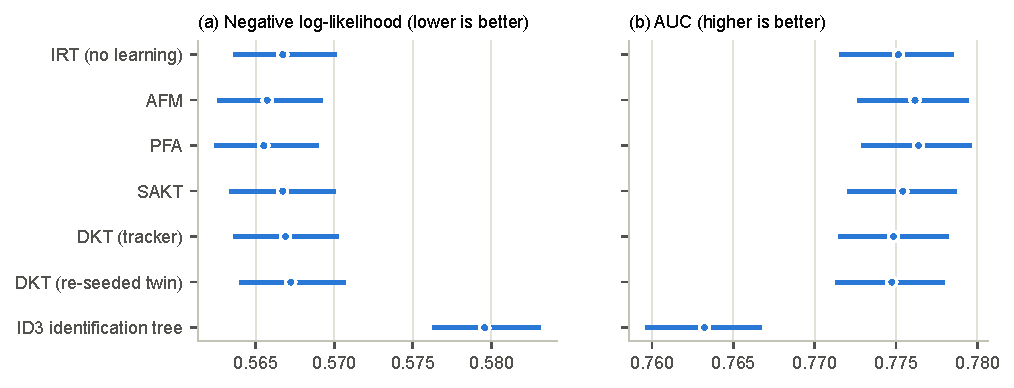
\includegraphics[width=\linewidth]{figures/fig_forecast.pdf}
\caption{Forecast accuracy on held-out learners. (a) Negative log-likelihood and (b) AUC of first-attempt forecasts for the 926 test learners (112,950 predictions); bars are 95\% learner-bootstrap intervals. The six statistical learner models overlap; the interpretable identification tree is somewhat less accurate.}
\label{fig:forecast}
\end{figure}

\subsection{Policies look strong in the simulator they were trained in}\label{sec:res-insim}

In the training simulator DKT-A, the KT-reward agents produced the largest gains: PPO improved the expected post-test by $+$28.58 pp and DQN by $+$14.59 pp over ten problems, against $+$1.42 pp for random selection; the one-step greedy maximiser of the tracker reached $+$15.31 pp (\cref{tab:matrix}). Agents trained in the AFM world or on mixed worlds also scored well in DKT-A (e.g.\ $+$13.11 pp for mixed-world DQN). Read in isolation, as is common in KT-simulator evaluations, these numbers would suggest a large benefit of reinforcement learning. They are, however, almost entirely drift: in DKT-A, where outcomes are generated by the tracker itself, the surprise term of \cref{eq:decomposition} averaged between $-$0.70 and 0.00 pp across the 14 policies (at most 2.3 Monte Carlo standard errors from zero; outcome streams are shared across policies), whereas PPO's accumulated drift was 29.0 pp, as \cref{prop:insim} predicts (exploratory check).

\begin{table*}[t]
\centering
\caption{World-measured post-test gain (percentage points over ten problems) of every policy in every evaluation world.}
\label{tab:matrix}
\footnotesize
\resizebox{\textwidth}{!}{%
\begin{tabular}{lrrrrrrrrr}
\toprule
Policy & DKT-A$^\dagger$ & AFM-A$^\dagger$ & DKT-A twin & DKT-B & SAKT-B & AFM-B & PFA-B & ZPD-B & IRT-B \\
\midrule
Random & 1.42 & 1.83 & 3.33 & 1.31 & 3.36 & 1.72 & 1.63 & 1.93 & 0.00 \\
Easy-to-hard curriculum & 3.51 & 0.54 & $-$2.12 & 2.34 & 14.17 & 0.53 & 0.63 & 0.52 & 0.00 \\
Weakest skill & 4.92 & 1.30 & 1.93 & 5.15 & 3.48 & 0.97 & 0.95 & 0.92 & 0.00 \\
Target success 0.5 & $-$0.86 & 1.75 & 2.58 & $-$0.97 & 2.32 & 1.66 & 1.51 & 2.18 & 0.00 \\
Target success 0.7 & 4.04 & 1.88 & 4.45 & $-$1.23 & 6.88 & 1.92 & 2.03 & 2.13 & 0.00 \\
Easiest first & 0.60 & 0.91 & 8.15 & 5.12 & 8.31 & 0.86 & 0.84 & 0.70 & 0.00 \\
Hardest first & 3.31 & 2.62 & 7.30 & 2.16 & 0.49 & 2.72 & 2.19 & 1.37 & 0.00 \\
Greedy on tracker & 15.31 & 2.02 & 9.00 & $-$2.99 & 5.70 & 2.35 & 2.42 & 2.00 & 0.00 \\
DQN (DKT reward) & 14.59 & 1.72 & 10.46 & 7.57 & 4.10 & 1.84 & 1.82 & 1.68 & 0.00 \\
PPO (DKT reward) & 28.58 & 1.65 & 13.40 & 2.71 & 9.24 & 2.04 & 1.97 & 1.88 & 0.00 \\
DQN (AFM world) & 5.06 & 3.07 & 4.48 & 0.46 & 5.27 & 3.24 & 3.35 & 2.59 & 0.00 \\
PPO (AFM world) & 7.15 & 3.05 & 7.95 & 0.00 & 2.83 & 3.14 & 3.34 & 2.30 & 0.00 \\
DQN (mixed worlds) & 13.11 & 1.92 & 7.22 & 1.63 & 7.52 & 2.11 & 1.94 & 2.09 & 0.00 \\
PPO (mixed worlds) & 11.54 & 2.76 & 5.89 & 1.98 & 5.72 & 3.07 & 3.08 & 2.25 & 0.00 \\
One-step oracle & -- & 3.20 & -- & -- & -- & 3.48 & 3.97 & 3.64 & 0.00 \\
\bottomrule
\end{tabular}}
\par\smallskip
\begin{minipage}{\textwidth}\footnotesize
\textit{Note.} Averages over 926 evaluation episodes and, for learned agents, three training seeds. $^\dagger$Training worlds. DKT and SAKT worlds are measured by their own predictions; AFM, PFA and ZPD worlds by the latent state; IRT-B has no learning, so every true gain is zero. The 95\% intervals are given in the supplementary file \texttt{evaluation\_matrix\_long.csv}.
\end{minipage}
\end{table*}

\subsection{H1: the in-simulator advantage does not survive independent worlds}\label{sec:res-h1}

Relative to random selection, DQN with the DKT reward gained $+$13.17 pp [12.56, 13.73] in DKT-A, but $+$7.12 pp in the re-seeded twin, $+$6.26 pp in DKT-B, $+$0.74 pp in SAKT-B, and $+$0.12, $+$0.19 and $-$0.25 pp in the latent AFM-B, PFA-B and ZPD-B worlds. For PPO the in-simulator advantage was $+$27.16 pp [26.54, 27.74], against $+$10.07, $+$1.40, $+$5.87, $+$0.32, $+$0.34 and $-$0.05 pp in the same six worlds. Every in-simulator-minus-independent difference was positive with an interval excluding zero (smallest: DQN versus the twin, $+$6.04 pp [5.27, 6.80]), supporting H1. In an exploratory comparison, policy rankings in DKT-A were only weakly related to rankings in the other worlds (Kendall $\tau$ = 0.49 with the twin, 0.05 with DKT-B, 0.23 with SAKT-B, 0.27 with AFM-B, 0.27 with PFA-B and 0.08 with ZPD-B). Neural worlds also disagreed with each other: the easy-to-hard curriculum gained 14.17 pp in SAKT-B but $-$2.12 pp in the DKT twin, where random selection gained 3.33 pp (\cref{fig:matrix}).

\begin{figure}[t]
\centering
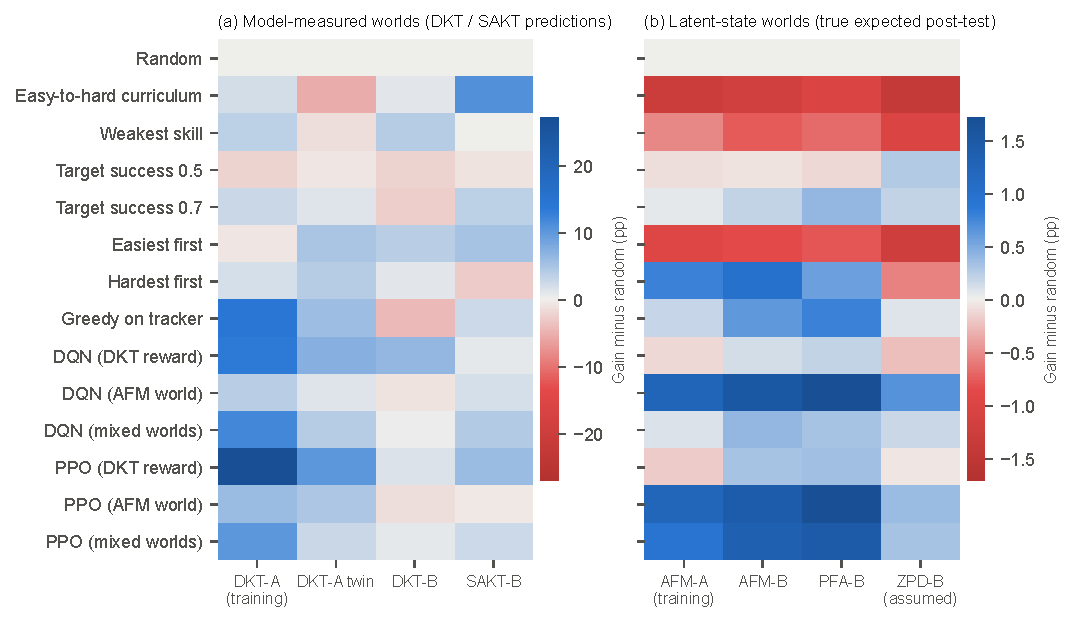
\includegraphics[width=\linewidth]{figures/fig_evaluation_matrix.pdf}
\caption{Gain relative to random selection in each world. (a) Worlds measured by a neural KT model's own predictions; (b) worlds with a known latent state. Blue cells: more simulated post-test gain than random; red cells: less. Colour scales differ between panels; values and 95\% intervals are in the supplementary file \texttt{evaluation\_matrix\_long.csv}.}
\label{fig:matrix}
\end{figure}

\subsection{H2 and H3: large gains are reported where no learning is possible}\label{sec:res-h2}

In the negative-control world IRT-B, the true post-test gain is exactly zero for every policy by construction. The deployed DKT tracker nevertheless reported gains of $+$12.57 pp [11.97, 13.19] for the greedy maximiser, $+$12.79 pp [12.17, 13.42] for DQN and $+$25.72 pp [25.06, 26.38] for PPO, supporting H2 (\cref{fig:phantom}). The reported gain depended strongly on the policy: it was $+$1.76 pp for random selection and $+$5.56 pp for the AFM-trained DQN. Across the 14 non-oracle policies, the gain in the training simulator and the phantom gain in the no-learning world were almost perfectly rank-correlated (Spearman $\rho$ = 0.960), supporting H3 (\cref{fig:insim}): the ranking produced by the standard in-simulator evaluation is essentially the ranking of how much learning the tracker attributes to a policy's problem choices when there is none. Other models fitted on A were far less affected (exploratory; \cref{tab:observers}): in IRT-B, AFM and PFA reported gains of at most 2.91 and 2.26 pp for any of these policies, and the static IRT model reported between $-$0.29 and 0.07 pp, that is, essentially none.

\begin{figure}[t]
\centering
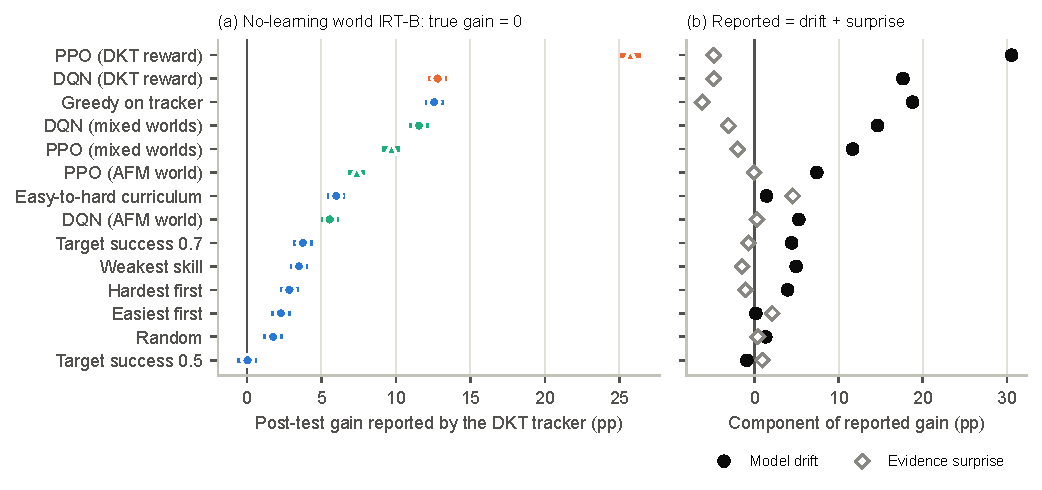
\includegraphics[width=\linewidth]{figures/fig_phantom_gain.pdf}
\caption{Negative control. (a) Post-test gain reported by the DKT tracker in the no-learning world IRT-B, where the true gain of every policy is zero (95\% intervals). (b) Exact decomposition of the reported gain into the tracker's drift and evidence surprise (\cref{eq:decomposition}).}
\label{fig:phantom}
\end{figure}

\begin{figure}[t]
\centering
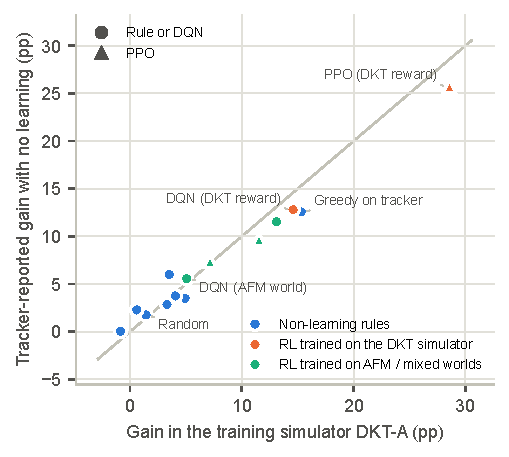
\includegraphics[width=0.62\linewidth]{figures/fig_in_sim_vs_phantom.pdf}
\caption{In-simulator gain in DKT-A against the phantom gain reported by the tracker in the no-learning world IRT-B for 14 policies (Spearman $\rho$ = 0.960). The grey diagonal is $y=x$; triangles are PPO agents.}
\label{fig:insim}
\end{figure}

\subsection{H4: where the phantom gain comes from}\label{sec:res-h4}

The decomposition in \cref{eq:decomposition} attributes the phantom gains to drift: in IRT-B, the tracker's own expected forecast change summed to $+$30.55 pp for PPO, $+$17.65 pp for DQN and $+$18.79 pp for the greedy maximiser, partly offset by negative surprise because the world was less favourable than the tracker expected. The learning implied by a single practice problem was far more dispersed for the neural models than for the models with explicit learning terms (\cref{fig:implied}): the standard deviation of per-problem drift was 3.31 pp for DKT, 3.15 for its twin and 2.01 for SAKT, against 0.20 for AFM, 0.16 for PFA and exactly 0.00 for IRT, as \cref{prop:nodrift} requires. The DKT--AFM difference was 3.11 pp [3.06, 3.16], supporting H4. In exploratory analyses, the two DKTs, which forecast equally well, agreed only weakly on which problems ``teach'' (Spearman $\rho$ = 0.35 [0.34, 0.36]), and DKT drift was higher for frequently attempted problems ($\rho$ = 0.32) and for easier problems ($\rho$ = $-$0.26 with IRT difficulty) but unrelated to typical course position ($\rho$ = $-$0.09).

Along learners' own next ten real interactions (905 learners; exploratory), the tracker's post-test forecast moved on average by only $+$0.41 pp, although the absolute movement averaged 9.43 pp, compared with 2.42 pp for IRT. On the sequences that learners actually followed, DKT's drift therefore largely cancels out; only when a policy selects problems for their drift does it accumulate into double-digit gains.

\begin{figure}[t]
\centering
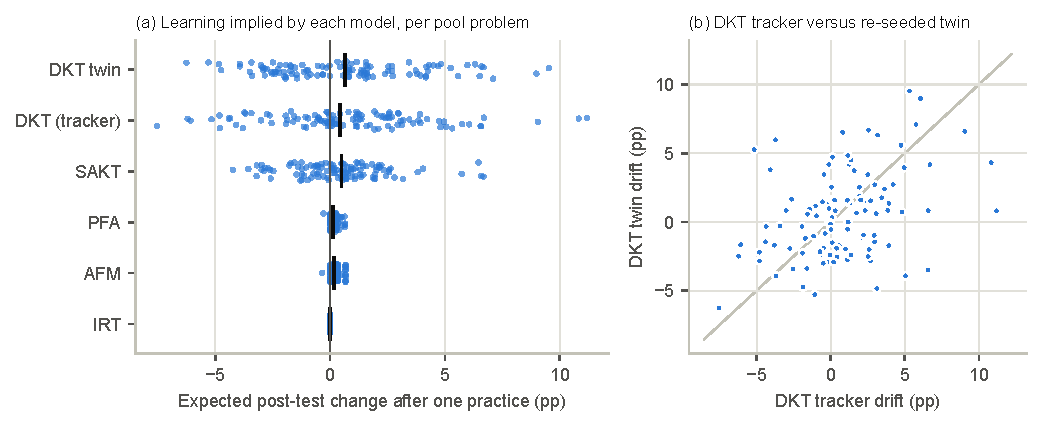
\includegraphics[width=\linewidth]{figures/fig_implied_learning.pdf}
\caption{Learning implied by each model. (a) Expected post-test change after one practice of each pool problem (drift), averaged over 300 start states; vertical bars are medians. (b) Drift of the DKT tracker against its re-seeded twin (Spearman $\rho$ = 0.35); the grey diagonal is $y=x$.}
\label{fig:implied}
\end{figure}

\subsection{Exploratory: which policies transfer}\label{sec:res-latent}

In the latent-state worlds the spread between policies was small but consistent (\cref{fig:effort}). Agents trained in the AFM world were the best non-privileged policies: in AFM-B the AFM-trained DQN gained 3.24 pp and PPO 3.14 pp, against 1.72 pp for random and 3.48 pp for the privileged one-step oracle; in PFA-B the corresponding values were 3.35, 3.34, 1.63 and 3.97 pp. In the assumed desirable-difficulty world ZPD-B the margin was smaller (2.59 and 2.30 against 1.93 pp). Their worst-case advantage over random across the three latent worlds was $+$0.66 pp for DQN and $+$0.37 pp for PPO, the largest of all policies, whereas the KT-reward agents had worst cases of $-$0.25 and $-$0.05 pp; PPO trained on mixed worlds came close ($+$0.32 pp). The AFM-trained agents also needed fewer extra submissions (6.4 and 5.0 per ten problems in AFM-B, against 10.8 for random).

This robustness has a clear limit. AFM-B, PFA-B and ZPD-B share the additive logistic structure of the AFM training world, so transfer among them is partly by construction. In the neural worlds, which do not share that structure, the AFM-trained agents' advantage over random ranged from $-$1.31 to $+$4.62 pp and was negative in DKT-B ($-$0.86 and $-$1.31 pp). Rules that targeted a predicted success of 0.7 were slightly better than random in every latent world (worst case $+$0.20 pp), whereas the easy-to-hard curriculum and easiest-first rules were consistently the worst in the latent worlds, spending practice on problems the learner would already solve.

\begin{figure}[t]
\centering
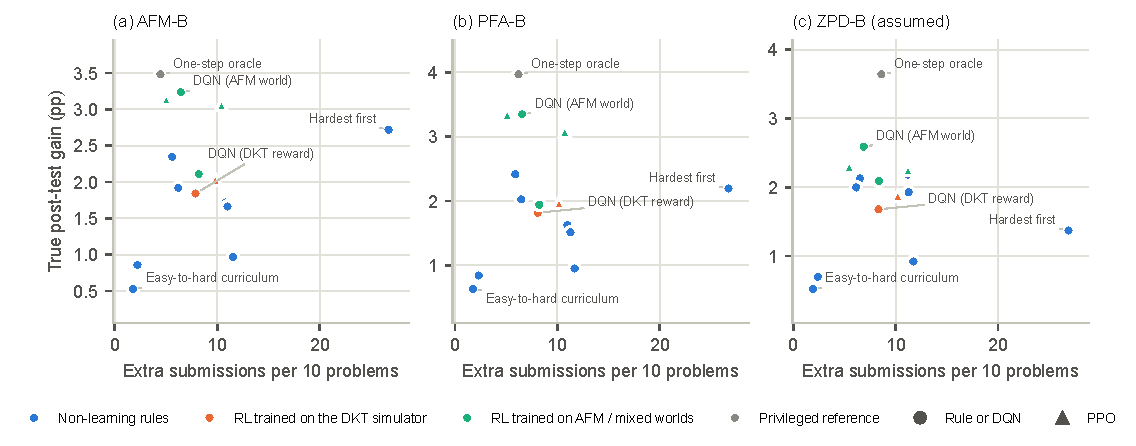
\includegraphics[width=\linewidth]{figures/fig_gain_effort.pdf}
\caption{True post-test gain against extra submissions per ten problems in the three latent worlds fitted or constructed from partition B: (a) AFM-B, (b) PFA-B and (c) the assumed desirable-difficulty world ZPD-B. Colours distinguish policy families and triangles mark PPO agents.}
\label{fig:effort}
\end{figure}

\section{Discussion}\label{sec:discussion}

\subsection{What the in-simulator gain measures}

The central finding is that, on real programming data, a policy's gain inside a KT simulator mainly measures how much learning the simulator's model \emph{believes} its problem choices produce, not how much a learner would learn. \Cref{prop:insim} makes this precise: when a KT model is both the simulator and the yardstick, the expected reported gain of any policy is its accumulated drift, and the empirical surprise in DKT-A was indeed negligible. Six learner models with equivalent forecasting accuracy implied very different learning: the explicit-learning models attributed small, homogeneous gains to practice, whereas the two DKTs attributed gains of several percentage points to single problems, in directions that a second random seed reproduced only weakly. This is an instance of underspecification \citep{damour2022underspecification}: the data constrain the next-step forecast, which all models match, but not the counterfactual consequences of practice sequences that learners never followed. It extends the observation that student models of similar accuracy can prescribe different amounts of practice \citep{lee2012individualizing,rollinson2015predictive} from mastery decisions to optimised sequencing policies, where the discrepancy is amplified rather than merely exposed. Reinforcement learning is an efficient search for exactly such sequences. The more capable optimiser (PPO) exploited the DKT reward most, reaching an in-simulator gain about twice that of DQN and a phantom gain of the same size in the no-learning world.

Two further observations sharpen the interpretation. First, for a given policy the tracker's reported gain varied little across the nine worlds---for PPO with the DKT reward between 25.7 and 28.6 pp, for random selection between 0.6 and 2.6 pp: its value is fixed mostly by which problems the policy selects, not by how the simulated learner responds. Second, along learners' actual continuations DKT's drift averaged out; its forecasts were volatile, as reported for DKT before \citep{yeung2018dktplus}, but not systematically biased there. The problem arises off the data distribution, where a policy compounds drift step after step. Predictive validation on logged sequences cannot detect this failure, which is why models that were indistinguishable in \cref{tab:forecast} could disagree about policies.

\subsection{Relation to model exploitation and reward over-optimisation}

The phantom gain is the educational counterpart of model exploitation in model-based RL and of reward over-optimisation: an agent optimised against a learned model finds the actions for which the model is most optimistic \citep{kurutach2018metrpo,janner2019trust,gao2023scaling,skalse2022reward}. KT--RL recommenders are particularly exposed because the same learned model provides dynamics, reward and evaluation, so an evaluation inside that model cannot reveal the exploitation. Remedies developed in model-based RL suggest testable designs for educational recommenders: penalising the disagreement of an ensemble of trackers, of which our re-seeded twin is a minimal instance \citep{kurutach2018metrpo,yu2020mopo}; restricting planning to short horizons or well-supported problems \citep{janner2019trust}; or constraining the learner model so that its drift is interpretable and monotone \citep{zhang2023cmkt}. We did not evaluate these remedies, and whether they would recover real learning gains is an open question.

\subsection{Implications for the evaluation of adaptive recommenders}

Our results do not show that the published systems we build on are wrong; we did not reproduce their tasks, rewards or datasets. They show that a design shared by many of them---training and scoring a policy with the same fitted KT model, or with models fitted to the same logs---can report large improvements for policies that teach nothing. We therefore suggest four inexpensive checks for simulator-based studies of exercise recommendation. (i) Report a \emph{negative control}: evaluate every policy in a world without learning in which the true gain is known to be zero, and report the tracker's claimed gain there. (ii) Report the \emph{drift decomposition} of \cref{eq:decomposition}, which requires only the tracker and exposes gains that the model expects from itself. (iii) Evaluate in \emph{independently fitted worlds} with different learning structures and learners, following the robust evaluation matrix \citep{doroudi2017rem}, including at least one world whose learning parameters are explicit. (iv) Re-fit the tracker with a different seed and report the agreement of implied learning. None of these checks needs student data beyond the logs already used. Because RL results vary across training seeds, such checks should be reported per seed or with seed-level uncertainty \citep{henderson2018matters,agarwal2021precipice}.

\subsection{What reinforcement learning can offer}

Reinforcement learning was not useless. When the training world had an explicit, interpretable learning structure (AFM), DQN and PPO learned policies that transferred to independently fitted AFM and PFA worlds and to a world with a different, assumed learning law, approaching a privileged one-step oracle while spending fewer submissions than random selection. This agrees with the observation of \citet{doroudi2019reward} that policies derived from theory-constrained models are more trustworthy than policies derived from unconstrained data-driven models. The evidence is nevertheless limited: the gains were modest---1.4 to 1.7 pp of expected post-test success over random selection across ten problems in AFM-B and PFA-B---they remain simulator quantities, the latent worlds share the AFM world's structure, and the same agents did not beat random selection in DKT-B. Rules that target a moderate predicted success (0.7) were also robust, whereas an easy-to-hard curriculum and easiest-first selection, the ``too easy'' extreme of the zone-of-proximal-development argument in the course brief, were consistently the least effective in the latent worlds.

\subsection{Limitations}

All policy outcomes are simulated. The latent worlds are fitted to observational logs of one platform and one course family; their learning coefficients are associations adjusted for ability and problem difficulty, not causal effects, and the ZPD world is an assumption. Because the latent worlds share an additive logistic structure, the robustness of agents trained in the AFM world is conditional on that structure. The skill grouping is ours, and pointers, although prominent in the course brief, were represented by only one pool problem because few pointer problems reached the 5\% support threshold. Effort is measured by submissions, not time on task. We studied first-attempt outcomes, a ten-problem horizon and a single effort weight; longer horizons, other rewards and other pools may change magnitudes, and we did not run sensitivity analyses on these choices. Each agent was trained with three seeds, and intervals condition on these seeds and on the fitted models; they are not adjusted for multiplicity, although all pre-registered contrasts are reported, and the rank correlations are computed over policies that are not independent of each other. The data come from one university's online judge, so generalisation to other languages, course designs and learner populations is untested. Finally, we did not test any policy with students; the evidence concerns the validity of simulator-based evaluation and the relative robustness of policies across plausible worlds, not learning gains of real learners.

\section{Conclusion}\label{sec:conclusion}

We built and evaluated an adaptive exercise recommender for C programming entirely from real learner logs: learner models including DKT and an entropy-based identification tree, a sequential decision problem whose reward combines post-test improvement and solving effort, and DQN and PPO agents. The learner models forecast equally well, yet the agents trained against the DKT simulator obtained large gains that did not survive independently fitted worlds and that the tracker also reported when no learning was possible. We showed that such in-simulator gains are, in expectation, the tracker's accumulated drift---learning the model promises itself---which a coherent model without learning never reports and which a re-seeded DKT did not reproduce. Agents trained with an explicit learning model transferred best within the family of latent worlds, but not to neural worlds. For researchers and developers of adaptive recommenders, the practical message is to accompany any simulator-based evaluation with a negative-control world, the drift decomposition and independently fitted worlds, and to treat in-simulator gains of optimised policies with suspicion until these checks are passed. Replication on other datasets, sensitivity analyses of the decision problem and, ultimately, a controlled study with students are needed to establish whether the robust policies help real learners; our pipeline and application are designed to support such work.

\appendix
\section{Proofs}\label{app:proofs}

\paragraph{Proof of \cref{prop:nodrift}} Write $\bar p(\theta)=|\mathcal W|^{-1}\sum_{k\in\mathcal W}p(y=1\mid k,\theta)$ and $\pi_H$ for the posterior of $\theta$ after history $H$. The model's forecasts are posterior predictive, $\bar P_M(H)=\int\bar p(\theta)\,\pi_H(\mathrm d\theta)$ and $P_M(y\mid j,H)=\int p(y\mid j,\theta)\,\pi_H(\mathrm d\theta)$. Because $\theta$ does not change with practice and outcomes are conditionally independent given $\theta$, Bayes' rule gives $\pi_{H\oplus(j,y)}(\mathrm d\theta)=p(y\mid j,\theta)\,\pi_H(\mathrm d\theta)/P_M(y\mid j,H)$. Hence
\begin{align}
\sum_{y\in\{0,1\}}P_M(y\mid j,H)\,\bar P_M\bigl(H\oplus(j,y)\bigr)
&=\sum_{y\in\{0,1\}}\int\bar p(\theta)\,p(y\mid j,\theta)\,\pi_H(\mathrm d\theta)\notag\\
&=\int\bar p(\theta)\,\pi_H(\mathrm d\theta)=\bar P_M(H),
\end{align}
so $D_M(j,H)=0$. The argument holds for any prior, including the finite grid used for IRT in this study, whose per-problem drift was exactly zero (\cref{sec:res-h4}). $\square$

\paragraph{Proof of \cref{prop:insim}} Let $S_t=\bar P_M(H_{t+1})-\bar P_M(H_t)-D_M(j_t,H_t)$ be the surprise at step $t$. If $y_t$ is drawn from $P_M(\cdot\mid j_t,H_t)$, then by \cref{eq:drift}
\begin{align}
\mathbb E\bigl[S_t\mid H_t,j_t\bigr]
&=\sum_{y\in\{0,1\}}P_M(y\mid j_t,H_t)\,\bar P_M\bigl(H_t\oplus(j_t,y)\bigr)\notag\\
&\quad-\bar P_M(H_t)-D_M(j_t,H_t)=0.
\end{align}
The choice $j_t$ depends only on $H_t$ and on randomisation independent of future outcomes, so the tower property gives $\mathbb E[S_t]=0$ for every $t$. Taking expectations of \cref{eq:decomposition} yields the result. Combining both propositions, a coherent simulator without learning assigns an expected in-simulator gain of zero to every policy, and a simulator with learning ranks policies by the drift they accumulate. $\square$

\section{Implementation details}\label{app:impl}

\paragraph{Learner models} Logistic models: priors $\theta\sim\mathcal N(0,\sigma_\theta^2)$ with $\sigma_\theta\in\{0.4,0.5,0.6,0.75\}$ selected by inner-validation NLL, problem terms $\mathcal N(0,1)$, learning coefficients $\mathcal N(0,1)$; full-batch L-BFGS. DKT: embedding 32, LSTM 64, dropout 0.3 (0.1 on inputs), AdamW with weight decay $10^{-4}$, learning rate $10^{-3}$, batch 32, early stopping with patience 3 (maximum 30 epochs). SAKT: dimension 64, 4 heads, window 200, dropout 0.1. Problems attempted by at least 10 fitting learners receive their own parameters. ID3: minimum leaf size 200, minimum gain $10^{-3}$, maximum depth 6.

\paragraph{Agents} State: 109 predicted success values, 109 eligibility flags, 10 skill averages, post-test forecast and remaining horizon. Double DQN: two hidden layers of 256, replay 50,000, batch 256, learning rate $5\times10^{-4}$, soft target update $\tau=0.01$, $\varepsilon$ from 1 to 0.05 over half of training, $\gamma=0.99$. PPO: two hidden layers of 256 (tanh), learning rate $3\times10^{-4}$, 4 epochs, minibatch 128, clip 0.2, entropy 0.01, GAE $\lambda=0.95$. Each agent: 300 iterations of 64 parallel ten-step episodes; the final checkpoint is used; seeds 11, 23 and 37. Effort: after a failed first attempt, additional submissions follow a geometric distribution with the problem's mean from the world's partition (shrunk to the overall mean, capped at 10).

\section{Skill-level forecasting}\label{app:skills}

\begin{table}[H]
\centering
\caption{AUC by primary skill of the target problem (test learners, models fitted on A).}
\label{tab:skills}
\small
\resizebox{\linewidth}{!}{%
\begin{tabular}{lrrrrrrr}
\toprule
Skill & $n$ & Base rate & IRT & PFA & DKT & SAKT & ID3 \\
\midrule
Basic syntax, I/O and data types & 44,513 & 0.55 & 0.774 & 0.775 & 0.774 & 0.775 & 0.763 \\
Conditionals & 4,171 & 0.53 & 0.761 & 0.763 & 0.768 & 0.763 & 0.751 \\
Loops & 2,528 & 0.48 & 0.754 & 0.758 & 0.761 & 0.752 & 0.745 \\
Arrays & 2,440 & 0.50 & 0.789 & 0.791 & 0.790 & 0.788 & 0.780 \\
Strings & 5,999 & 0.53 & 0.731 & 0.733 & 0.729 & 0.731 & 0.716 \\
Pointers and linked lists & 444 & 0.66 & 0.701 & 0.705 & 0.699 & 0.691 & 0.709 \\
Bit operations and number bases & 9,219 & 0.50 & 0.764 & 0.766 & 0.764 & 0.766 & 0.750 \\
Arithmetic and number theory & 4,557 & 0.52 & 0.823 & 0.824 & 0.817 & 0.824 & 0.812 \\
Recursion, recurrence and divide-and-conquer & 3,344 & 0.57 & 0.789 & 0.790 & 0.784 & 0.783 & 0.777 \\
Sorting and searching & 5,433 & 0.44 & 0.755 & 0.757 & 0.749 & 0.749 & 0.737 \\
\bottomrule
\end{tabular}}
\end{table}

\section{Gains claimed by other models in the negative control}\label{app:observers}

\begin{table}[H]
\centering
\caption{Post-test gain (pp) that each A-fitted model would report after the same episodes in the no-learning world IRT-B (exploratory). True gain is zero.}
\label{tab:observers}
\small
\begin{tabular}{lrrrrr}
\toprule
Policy & DKT & SAKT & AFM & PFA & IRT \\
\midrule
Random & 1.76 & 3.69 & 1.73 & 1.40 & $-$0.14 \\
Easy-to-hard curriculum & 6.00 & 11.12 & 0.64 & 0.55 & 0.06 \\
Target success 0.7 & 3.75 & 5.28 & 1.62 & 1.20 & $-$0.25 \\
Greedy on tracker & 12.57 & 5.58 & 2.05 & 1.50 & $-$0.08 \\
DQN (DKT reward) & 12.79 & 3.87 & 1.21 & 0.81 & $-$0.27 \\
PPO (DKT reward) & 25.72 & 5.93 & 1.57 & 1.19 & $-$0.04 \\
DQN (AFM world) & 5.56 & 3.45 & 2.91 & 2.26 & $-$0.13 \\
PPO (AFM world) & 7.37 & 3.54 & 2.56 & 1.92 & $-$0.28 \\
\bottomrule
\end{tabular}
\end{table}

\section{Reproducibility}\label{app:repro}

Both protocols were locked before the evaluation population was loaded; the lock record lists SHA-256 hashes of protocols and code. Experiments ran through an append-only harness that snapshots protocol and source, records input and output hashes and refuses to overwrite a run. Run records: learner stage \texttt{10bf859c0486}\ldots, policy stage \texttt{167b9e90f3f3}\ldots\ (SHA-256 prefixes). Development and hyperparameter choices used a previously inspected cohort disjoint from the evaluation population. All numbers in this manuscript are inserted programmatically from the run outputs.

\section*{Data availability}
The ACcoding dataset is publicly available from its authors \citep{sun2026accodingdata,chen2024accoding}. Code, locked protocols, run records, aggregate results and the tables behind every figure will be deposited in a public repository upon acceptance (an anonymised copy is available to reviewers on request); learner-level derived files are not redistributed.

\section*{Ethics statement}
This is a secondary analysis of a public, anonymised dataset. No new data were collected and no learner was contacted or assigned to a condition.

\section*{Declaration of generative AI and AI-assisted technologies in the manuscript preparation process}
During the preparation of this work the author(s) used Claude (Anthropic), an AI assistant, in order to write and run analysis and plotting code and to draft and edit the text. After using this tool, the author(s) reviewed and edited the content as needed and take(s) full responsibility for the content of the published article. \emph{[Authors: confirm or amend this statement so that it matches your actual use before submission.]}

\begin{thebibliography}{73}
\expandafter\ifx\csname url\endcsname\relax
  \def\url#1{\texttt{#1}}\fi
\bibitem[{Abdelrahman et~al.(2023)Abdelrahman, Wang, and Nunes}]{abdelrahman2023survey}
Abdelrahman, G., Wang, Q., \& Nunes, B. (2023). Knowledge tracing: A survey. \textit{ACM Computing Surveys}, \textit{55}(11), 1--37. \url{https://doi.org/10.1145/3569576}

\bibitem[{Agarwal et~al.(2021)Agarwal, Schwarzer, Castro, Courville, and Bellemare}]{agarwal2021precipice}
Agarwal, R., Schwarzer, M., Castro, P. S., Courville, A., \& Bellemare, M. G. (2021). Deep reinforcement learning at the edge of the statistical precipice. In \textit{Advances in Neural Information Processing Systems} (Vol.~34, pp.~29304--29320). Curran Associates.

\bibitem[{Ai et~al.(2019)Ai, Chen, Guo, Zhao, Wang, Fu, and Wang}]{ai2019cdkt}
Ai, F., Chen, Y., Guo, Y., Zhao, Y., Wang, Z., Fu, G., \& Wang, G. (2019). Concept-aware deep knowledge tracing and exercise recommendation in an online learning system. In \textit{Proceedings of the 12th International Conference on Educational Data Mining} (pp.~240--245). International Educational Data Mining Society. \url{https://eric.ed.gov/?id=ED599194}

\bibitem[{Amodei et~al.(2016)Amodei, Olah, Steinhardt, Christiano, Schulman, and Man{\'e}}]{amodei2016concrete}
Amodei, D., Olah, C., Steinhardt, J., Christiano, P., Schulman, J., \& Man{\'e}, D. (2016). \textit{Concrete problems in AI safety} [Preprint]. arXiv. \url{https://doi.org/10.48550/arXiv.1606.06565}

\bibitem[{Arnold et~al.(2016)Arnold, Ercumen, Benjamin-Chung, and Colford}]{arnold2016negative}
Arnold, B. F., Ercumen, A., Benjamin-Chung, J., \& Colford, J. M. (2016). Brief report: Negative controls to detect selection bias and measurement bias in epidemiologic studies. \textit{Epidemiology}, \textit{27}(5), 637--641. \url{https://doi.org/10.1097/EDE.0000000000000504}

\bibitem[{Bassen et~al.(2020)Bassen, Balaji, Schaarschmidt, Thille, Painter, Zimmaro, Games, Fast, and Mitchell}]{bassen2020chi}
Bassen, J., Balaji, B., Schaarschmidt, M., Thille, C., Painter, J., Zimmaro, D., Games, A., Fast, E., \& Mitchell, J. C. (2020). Reinforcement learning for the adaptive scheduling of educational activities. In \textit{Proceedings of the 2020 CHI Conference on Human Factors in Computing Systems} (pp.~1--12). ACM. \url{https://doi.org/10.1145/3313831.3376518}

\bibitem[{Breiman(2001)Breiman}]{breiman2001two}
Breiman, L. (2001). Statistical modeling: The two cultures. \textit{Statistical Science}, \textit{16}(3), 199--231. \url{https://doi.org/10.1214/ss/1009213726}

\bibitem[{Brusilovsky and Mill{\'a}n(2007)Brusilovsky and Mill{\'a}n}]{brusilovsky2007user}
Brusilovsky, P., \& Mill{\'a}n, E. (2007). User models for adaptive hypermedia and adaptive educational systems. In P. Brusilovsky, A. Kobsa, \& W. Nejdl (Eds.), \textit{The adaptive web: Methods and strategies of web personalization} (Lecture Notes in Computer Science, Vol.~4321, pp.~3--53). Springer. \url{https://doi.org/10.1007/978-3-540-72079-9_1}

\bibitem[{Cen et~al.(2006)Cen, Koedinger, and Junker}]{cen2006lfa}
Cen, H., Koedinger, K. R., \& Junker, B. (2006). Learning factors analysis -- A general method for cognitive model evaluation and improvement. In \textit{Intelligent Tutoring Systems: 8th International Conference, ITS 2006} (Lecture Notes in Computer Science, Vol.~4053, pp.~164--175). Springer. \url{https://doi.org/10.1007/11774303_17}

\bibitem[{Chen et~al.(2024)Chen, Huang, Liu, Yu, Meng, Mo, Zhang, and Song}]{chen2024accoding}
Chen, K., Huang, F., Liu, Z., Yu, H., Meng, L., Mo, S., Zhang, L., \& Song, Y. (2024). ACcoding: A graph-based dataset for online judge programming. \textit{Scientific Data}, \textit{11}, Article 548. \url{https://doi.org/10.1038/s41597-024-03392-z}

\bibitem[{Chen et~al.(2023)Chen, Shen, Xia, Jin, Song, Zhang, Liu, Zhu, Tang, Dong, Xia, and Yu}]{chen2023src}
Chen, X., Shen, J., Xia, W., Jin, J., Song, Y., Zhang, W., Liu, W., Zhu, M., Tang, R., Dong, K., Xia, D., \& Yu, Y. (2023). Set-to-sequence ranking-based concept-aware learning path recommendation. \textit{Proceedings of the AAAI Conference on Artificial Intelligence}, \textit{37}(4), 5027--5035. \url{https://doi.org/10.1609/aaai.v37i4.25630}

\bibitem[{Cheng et~al.(2026)Cheng, Zhuang, Xie, Wang, Liu, Guan, Fang, and Pan}]{cheng2026unier}
Cheng, X., Zhuang, G., Xie, Y., Wang, J., Liu, Y., Guan, Q., Fang, L., \& Pan, S. (2026). \textit{UniER: A unified benchmark for item-level and path-level exercise recommendation} [Preprint]. arXiv. \url{https://doi.org/10.48550/arXiv.2605.16750}

\bibitem[{Chi et~al.(2011)Chi, VanLehn, Litman, and Jordan}]{chi2011umuai}
Chi, M., VanLehn, K., Litman, D., \& Jordan, P. (2011). Empirically evaluating the application of reinforcement learning to the induction of effective and adaptive pedagogical strategies. \textit{User Modeling and User-Adapted Interaction}, \textit{21}(1--2), 137--180. \url{https://doi.org/10.1007/s11257-010-9093-1}

\bibitem[{Clement et~al.(2015)Clement, Roy, Oudeyer, and Lopes}]{clement2015bandits}
Clement, B., Roy, D., Oudeyer, P.-Y., \& Lopes, M. (2015). Multi-armed bandits for intelligent tutoring systems. \textit{Journal of Educational Data Mining}, \textit{7}(2), 20--48. \url{https://doi.org/10.5281/zenodo.3554667}

\bibitem[{Corbett and Anderson(1994)Corbett and Anderson}]{corbett1994bkt}
Corbett, A. T., \& Anderson, J. R. (1994). Knowledge tracing: Modeling the acquisition of procedural knowledge. \textit{User Modeling and User-Adapted Interaction}, \textit{4}(4), 253--278. \url{https://doi.org/10.1007/BF01099821}

\bibitem[{D'Amour et~al.(2022)D'Amour, Heller, Moldovan, Adlam, Alipanahi, Beutel, Chen, Deaton, Eisenstein, Hoffman, Hormozdiari, Houlsby, Hou, Jerfel, Karthikesalingam, Lucic, Ma, McLean, Mincu, Mitani, Montanari, Nado, Natarajan, Nielson, Osborne, Raman, Ramasamy, Sayres, Schrouff, Seneviratne, Sequeira, Suresh, Veitch, Vladymyrov, Wang, Webster, Yadlowsky, Yun, Zhai, and Sculley}]{damour2022underspecification}
D'Amour, A., Heller, K., Moldovan, D., Adlam, B., Alipanahi, B., Beutel, A., Chen, C., Deaton, J., Eisenstein, J., Hoffman, M. D., Hormozdiari, F., Houlsby, N., Hou, S., Jerfel, G., Karthikesalingam, A., Lucic, M., Ma, Y., McLean, C., Mincu, D., \ldots\ Sculley, D. (2022). Underspecification presents challenges for credibility in modern machine learning. \textit{Journal of Machine Learning Research}, \textit{23}(226), 1--61. \url{https://jmlr.org/papers/v23/20-1335.html}

\bibitem[{Doroudi et~al.(2017)Doroudi, Aleven, and Brunskill}]{doroudi2017rem}
Doroudi, S., Aleven, V., \& Brunskill, E. (2017). Robust evaluation matrix: Towards a more principled offline exploration of instructional policies. In \textit{Proceedings of the Fourth ACM Conference on Learning @ Scale} (pp.~3--12). ACM. \url{https://doi.org/10.1145/3051457.3051463}

\bibitem[{Doroudi et~al.(2019)Doroudi, Aleven, and Brunskill}]{doroudi2019reward}
Doroudi, S., Aleven, V., \& Brunskill, E. (2019). Where's the reward? A review of reinforcement learning for instructional sequencing. \textit{International Journal of Artificial Intelligence in Education}, \textit{29}(4), 568--620. \url{https://doi.org/10.1007/s40593-019-00187-x}

\bibitem[{Doroudi and Brunskill(2017)Doroudi and Brunskill}]{doroudi2017identifiability}
Doroudi, S., \& Brunskill, E. (2017). The misidentified identifiability problem of Bayesian knowledge tracing. In \textit{Proceedings of the 10th International Conference on Educational Data Mining} (pp.~143--149). International Educational Data Mining Society. \url{https://eric.ed.gov/?id=ED596611}

\bibitem[{Doroudi and Brunskill(2019)Doroudi and Brunskill}]{doroudi2019fairer}
Doroudi, S., \& Brunskill, E. (2019). Fairer but not fair enough: On the equitability of knowledge tracing. In \textit{Proceedings of the 9th International Conference on Learning Analytics \& Knowledge} (pp.~335--339). ACM. \url{https://doi.org/10.1145/3303772.3303838}

\bibitem[{Dulac-Arnold et~al.(2021)Dulac-Arnold, Levine, Mankowitz, Li, Paduraru, Gowal, and Hester}]{dulacarnold2021challenges}
Dulac-Arnold, G., Levine, N., Mankowitz, D. J., Li, J., Paduraru, C., Gowal, S., \& Hester, T. (2021). Challenges of real-world reinforcement learning: Definitions, benchmarks and analysis. \textit{Machine Learning}, \textit{110}(9), 2419--2468. \url{https://doi.org/10.1007/s10994-021-05961-4}

\bibitem[{Efron and Tibshirani(1993)Efron and Tibshirani}]{efron1993bootstrap}
Efron, B., \& Tibshirani, R. J. (1993). \textit{An introduction to the bootstrap}. Chapman \& Hall.

\bibitem[{Gao et~al.(2023)Gao, Schulman, and Hilton}]{gao2023scaling}
Gao, L., Schulman, J., \& Hilton, J. (2023). Scaling laws for reward model overoptimization. In \textit{Proceedings of the 40th International Conference on Machine Learning} (Proceedings of Machine Learning Research, Vol.~202, pp.~10835--10866). PMLR. \url{https://proceedings.mlr.press/v202/gao23h.html}

\bibitem[{Gervet et~al.(2020)Gervet, Koedinger, Schneider, and Mitchell}]{gervet2020deep}
Gervet, T., Koedinger, K., Schneider, J., \& Mitchell, T. (2020). When is deep learning the best approach to knowledge tracing? \textit{Journal of Educational Data Mining}, \textit{12}(3), 31--54. \url{https://doi.org/10.5281/zenodo.4143614}

\bibitem[{Ghosh et~al.(2020)Ghosh, Heffernan, and Lan}]{ghosh2020akt}
Ghosh, A., Heffernan, N., \& Lan, A. S. (2020). Context-aware attentive knowledge tracing. In \textit{Proceedings of the 26th ACM SIGKDD International Conference on Knowledge Discovery \& Data Mining} (pp.~2330--2339). ACM. \url{https://doi.org/10.1145/3394486.3403282}

\bibitem[{Gonz{\'a}lez-Brenes and Huang(2015)Gonz{\'a}lez-Brenes and Huang}]{gonzalezbrenes2015leopard}
Gonz{\'a}lez-Brenes, J. P., \& Huang, Y. (2015). Your model is predictive---but is it useful? Theoretical and empirical considerations of a new paradigm for adaptive tutoring evaluation. In \textit{Proceedings of the 8th International Conference on Educational Data Mining} (pp.~187--194). International Educational Data Mining Society. \url{https://eric.ed.gov/?id=ED560590}

\bibitem[{Henderson et~al.(2018)Henderson, Islam, Bachman, Pineau, Precup, and Meger}]{henderson2018matters}
Henderson, P., Islam, R., Bachman, P., Pineau, J., Precup, D., \& Meger, D. (2018). Deep reinforcement learning that matters. \textit{Proceedings of the AAAI Conference on Artificial Intelligence}, \textit{32}(1). \url{https://doi.org/10.1609/aaai.v32i1.11694}

\bibitem[{Hsiao et~al.(2010)Hsiao, Sosnovsky, and Brusilovsky}]{hsiao2010guiding}
Hsiao, I.-H., Sosnovsky, S., \& Brusilovsky, P. (2010). Guiding students to the right questions: Adaptive navigation support in an E-Learning system for Java programming. \textit{Journal of Computer Assisted Learning}, \textit{26}(4), 270--283. \url{https://doi.org/10.1111/j.1365-2729.2010.00365.x}

\bibitem[{Huang et~al.(2020)Huang, Oosterhuis, de Rijke, and van Hoof}]{huang2020keeping}
Huang, J., Oosterhuis, H., de Rijke, M., \& van Hoof, H. (2020). Keeping dataset biases out of the simulation: A debiased simulator for reinforcement learning based recommender systems. In \textit{Proceedings of the 14th ACM Conference on Recommender Systems} (pp.~190--199). ACM. \url{https://doi.org/10.1145/3383313.3412252}

\bibitem[{Huang et~al.(2015)Huang, Gonz{\'a}lez-Brenes, Kumar, and Brusilovsky}]{huang2015multifaceted}
Huang, Y., Gonz{\'a}lez-Brenes, J. P., Kumar, R., \& Brusilovsky, P. (2015). A framework for multifaceted evaluation of student models. In \textit{Proceedings of the 8th International Conference on Educational Data Mining} (pp.~203--210). International Educational Data Mining Society. \url{https://eric.ed.gov/?id=ED560517}

\bibitem[{Huang et~al.(2019)Huang, Liu, Zhai, Yin, Chen, Gao, and Hu}]{huang2019dre}
Huang, Z., Liu, Q., Zhai, C., Yin, Y., Chen, E., Gao, W., \& Hu, G. (2019). Exploring multi-objective exercise recommendations in online education systems. In \textit{Proceedings of the 28th ACM International Conference on Information and Knowledge Management} (pp.~1261--1270). ACM. \url{https://doi.org/10.1145/3357384.3357995}

\bibitem[{Janner et~al.(2019)Janner, Fu, Zhang, and Levine}]{janner2019trust}
Janner, M., Fu, J., Zhang, M., \& Levine, S. (2019). When to trust your model: Model-based policy optimization. In \textit{Advances in Neural Information Processing Systems} (Vol.~32). Curran Associates.

\bibitem[{Khajah et~al.(2016)Khajah, Lindsey, and Mozer}]{khajah2016deep}
Khajah, M., Lindsey, R. V., \& Mozer, M. C. (2016). How deep is knowledge tracing? In \textit{Proceedings of the 9th International Conference on Educational Data Mining} (pp.~94--101). International Educational Data Mining Society.

\bibitem[{Koedinger et~al.(2012)Koedinger, Corbett, and Perfetti}]{koedinger2012kli}
Koedinger, K. R., Corbett, A. T., \& Perfetti, C. (2012). The Knowledge-Learning-Instruction framework: Bridging the science-practice chasm to enhance robust student learning. \textit{Cognitive Science}, \textit{36}(5), 757--798. \url{https://doi.org/10.1111/j.1551-6709.2012.01245.x}

\bibitem[{Kurutach et~al.(2018)Kurutach, Clavera, Duan, Tamar, and Abbeel}]{kurutach2018metrpo}
Kurutach, T., Clavera, I., Duan, Y., Tamar, A., \& Abbeel, P. (2018). Model-ensemble trust-region policy optimization. In \textit{International Conference on Learning Representations}.

\bibitem[{Lee and Brunskill(2012)Lee and Brunskill}]{lee2012individualizing}
Lee, J. I., \& Brunskill, E. (2012). The impact on individualizing student models on necessary practice opportunities. In \textit{Proceedings of the 5th International Conference on Educational Data Mining} (pp.~118--125). International Educational Data Mining Society. \url{https://eric.ed.gov/?id=ED537193}

\bibitem[{Levine et~al.(2020)Levine, Kumar, Tucker, and Fu}]{levine2020offline}
Levine, S., Kumar, A., Tucker, G., \& Fu, J. (2020). \textit{Offline reinforcement learning: Tutorial, review, and perspectives on open problems} [Preprint]. arXiv. \url{https://doi.org/10.48550/arXiv.2005.01643}

\bibitem[{Li et~al.(2024)Li, Xia, Yin, Jin, and Yu}]{li2024pksd}
Li, Q., Xia, W., Yin, L., Jin, J., \& Yu, Y. (2024). Privileged knowledge state distillation for reinforcement learning-based educational path recommendation. In \textit{Proceedings of the 30th ACM SIGKDD Conference on Knowledge Discovery and Data Mining} (pp.~1621--1630). ACM. \url{https://doi.org/10.1145/3637528.3671872}

\bibitem[{Li et~al.(2023)Li, Xia, Yin, Shen, Rui, Zhang, Chen, Tang, and Yu}]{li2023gehrl}
Li, Q., Xia, W., Yin, L., Shen, J., Rui, R., Zhang, W., Chen, X., Tang, R., \& Yu, Y. (2023). Graph enhanced hierarchical reinforcement learning for goal-oriented learning path recommendation. In \textit{Proceedings of the 32nd ACM International Conference on Information and Knowledge Management} (pp.~1318--1327). ACM. \url{https://doi.org/10.1145/3583780.3614897}

\bibitem[{Lipsitch et~al.(2010)Lipsitch, Tchetgen Tchetgen, and Cohen}]{lipsitch2010negative}
Lipsitch, M., Tchetgen Tchetgen, E., \& Cohen, T. (2010). Negative controls: A tool for detecting confounding and bias in observational studies. \textit{Epidemiology}, \textit{21}(3), 383--388. \url{https://doi.org/10.1097/EDE.0b013e3181d61eeb}

\bibitem[{Liu et~al.(2019)Liu, Tong, Liu, Zhao, Chen, Ma, and Wang}]{liu2019cseal}
Liu, Q., Tong, S., Liu, C., Zhao, H., Chen, E., Ma, H., \& Wang, S. (2019). Exploiting cognitive structure for adaptive learning. In \textit{Proceedings of the 25th ACM SIGKDD International Conference on Knowledge Discovery \& Data Mining} (pp.~627--635). ACM. \url{https://doi.org/10.1145/3292500.3330922}

\bibitem[{Mandel et~al.(2014)Mandel, Liu, Levine, Brunskill, and Popovi{\'c}}]{mandel2014offline}
Mandel, T., Liu, Y.-E., Levine, S., Brunskill, E., \& Popovi{\'c}, Z. (2014). Offline policy evaluation across representations with applications to educational games. In \textit{Proceedings of the 2014 International Conference on Autonomous Agents and Multi-Agent Systems} (pp.~1077--1084). IFAAMAS. \url{https://doi.org/10.65109/tnvs8310}

\bibitem[{Mnih et~al.(2015)Mnih, Kavukcuoglu, Silver, Rusu, Veness, Bellemare, Graves, Riedmiller, Fidjeland, Ostrovski, Petersen, Beattie, Sadik, Antonoglou, King, Kumaran, Wierstra, Legg, and Hassabis}]{mnih2015dqn}
Mnih, V., Kavukcuoglu, K., Silver, D., Rusu, A. A., Veness, J., Bellemare, M. G., Graves, A., Riedmiller, M., Fidjeland, A. K., Ostrovski, G., Petersen, S., Beattie, C., Sadik, A., Antonoglou, I., King, H., Kumaran, D., Wierstra, D., Legg, S., \& Hassabis, D. (2015). Human-level control through deep reinforcement learning. \textit{Nature}, \textit{518}(7540), 529--533. \url{https://doi.org/10.1038/nature14236}

\bibitem[{Moerland et~al.(2023)Moerland, Broekens, Plaat, and Jonker}]{moerland2023mbrl}
Moerland, T. M., Broekens, J., Plaat, A., \& Jonker, C. M. (2023). Model-based reinforcement learning: A survey. \textit{Foundations and Trends in Machine Learning}, \textit{16}(1), 1--118. \url{https://doi.org/10.1561/2200000086}

\bibitem[{Ozyurt et~al.(2025)Ozyurt, Almaci, Feuerriegel, and Sachan}]{ozyurt2025exrec}
Ozyurt, Y., Almaci, T., Feuerriegel, S., \& Sachan, M. (2025). Personalized exercise recommendation with semantically-grounded knowledge tracing. In \textit{Advances in Neural Information Processing Systems} (Vol.~38, pp.~13019--13059). Curran Associates. \url{https://doi.org/10.52202/085713-0440}

\bibitem[{Pandey and Karypis(2019)Pandey and Karypis}]{pandey2019sakt}
Pandey, S., \& Karypis, G. (2019). A self-attentive model for knowledge tracing. In \textit{Proceedings of the 12th International Conference on Educational Data Mining} (pp.~384--389). International Educational Data Mining Society. \url{https://eric.ed.gov/?id=ED599186}

\bibitem[{Pavlik et~al.(2009)Pavlik, Cen, and Koedinger}]{pavlik2009pfa}
Pavlik, P. I., Cen, H., \& Koedinger, K. R. (2009). Performance factors analysis -- A new alternative to knowledge tracing. In \textit{Proceedings of the 14th International Conference on Artificial Intelligence in Education} (pp.~531--538). IOS Press.

\bibitem[{Pel{\'a}nek(2017)Pel{\'a}nek}]{pelanek2017learner}
Pel{\'a}nek, R. (2017). Bayesian knowledge tracing, logistic models, and beyond: An overview of learner modeling techniques. \textit{User Modeling and User-Adapted Interaction}, \textit{27}(3--5), 313--350. \url{https://doi.org/10.1007/s11257-017-9193-2}

\bibitem[{Piech et~al.(2015)Piech, Bassen, Huang, Ganguli, Sahami, Guibas, and Sohl-Dickstein}]{piech2015dkt}
Piech, C., Bassen, J., Huang, J., Ganguli, S., Sahami, M., Guibas, L. J., \& Sohl-Dickstein, J. (2015). Deep knowledge tracing. In \textit{Advances in Neural Information Processing Systems} (Vol.~28, pp.~505--513). Curran Associates.

\bibitem[{Press et~al.(2022)Press, Smith, and Lewis}]{press2022alibi}
Press, O., Smith, N. A., \& Lewis, M. (2022). Train short, test long: Attention with linear biases enables input length extrapolation. In \textit{International Conference on Learning Representations}.

\bibitem[{Quinlan(1986)Quinlan}]{quinlan1986id3}
Quinlan, J. R. (1986). Induction of decision trees. \textit{Machine Learning}, \textit{1}(1), 81--106. \url{https://doi.org/10.1007/BF00116251}

\bibitem[{Rafferty et~al.(2016)Rafferty, Brunskill, Griffiths, and Shafto}]{rafferty2016pomdp}
Rafferty, A. N., Brunskill, E., Griffiths, T. L., \& Shafto, P. (2016). Faster teaching via POMDP planning. \textit{Cognitive Science}, \textit{40}(6), 1290--1332. \url{https://doi.org/10.1111/cogs.12290}

\bibitem[{Riedmann et~al.(2025)Riedmann, Schaper, and Lugrin}]{riedmann2025rlreview}
Riedmann, A., Schaper, P., \& Lugrin, B. (2025). Reinforcement learning in education: A systematic literature review. \textit{International Journal of Artificial Intelligence in Education}, \textit{35}(5), 2669--2723. \url{https://doi.org/10.1007/s40593-025-00494-6}

\bibitem[{Rollinson and Brunskill(2015)Rollinson and Brunskill}]{rollinson2015predictive}
Rollinson, J., \& Brunskill, E. (2015). From predictive models to instructional policies. In \textit{Proceedings of the 8th International Conference on Educational Data Mining} (pp.~179--186). International Educational Data Mining Society. \url{https://eric.ed.gov/?id=ED560516}

\bibitem[{Ruan and Lu(2025)Ruan and Lu}]{ruan2025adaptive}
Ruan, S., \& Lu, K. (2025). Adaptive deep reinforcement learning for personalized learning pathways: A multimodal data-driven approach with real-time feedback optimization. \textit{Computers and Education: Artificial Intelligence}, \textit{9}, Article 100463. \url{https://doi.org/10.1016/j.caeai.2025.100463}

\bibitem[{Ruan et~al.(2024)Ruan, Nie, Steenbergen, He, Zhang, Guo, Liu, Dang Nguyen, Wang, Ying, Landay, and Brunskill}]{ruan2024rltutor}
Ruan, S., Nie, A., Steenbergen, W., He, J., Zhang, J. Q., Guo, M., Liu, Y., Dang Nguyen, K., Wang, C. Y., Ying, R., Landay, J. A., \& Brunskill, E. (2024). Reinforcement learning tutor better supported lower performers in a math task. \textit{Machine Learning}, \textit{113}(5), 3023--3048. \url{https://doi.org/10.1007/s10994-023-06423-9}

\bibitem[{Schulman et~al.(2017)Schulman, Wolski, Dhariwal, Radford, and Klimov}]{schulman2017ppo}
Schulman, J., Wolski, F., Dhariwal, P., Radford, A., \& Klimov, O. (2017). \textit{Proximal policy optimization algorithms} [Preprint]. arXiv. \url{https://doi.org/10.48550/arXiv.1707.06347}

\bibitem[{Shen et~al.(2018)Shen, Mostafavi, Barnes, and Chi}]{shen2018jedm}
Shen, S., Mostafavi, B., Barnes, T., \& Chi, M. (2018). Exploring induced pedagogical strategies through a Markov decision process framework: Lessons learned. \textit{Journal of Educational Data Mining}, \textit{10}(3), 27--68. \url{https://doi.org/10.5281/zenodo.3554713}

\bibitem[{Shi et~al.(2022)Shi, Chi, Barnes, and Price}]{shi2022codedkt}
Shi, Y., Chi, M., Barnes, T., \& Price, T. (2022). Code-DKT: A code-based knowledge tracing model for programming tasks. In \textit{Proceedings of the 15th International Conference on Educational Data Mining} (pp.~50--61). International Educational Data Mining Society. \url{https://doi.org/10.5281/zenodo.6853105}

\bibitem[{Singla et~al.(2021)Singla, Rafferty, Radanovic, and Heffernan}]{singla2021rleducation}
Singla, A., Rafferty, A. N., Radanovic, G., \& Heffernan, N. T. (2021). \textit{Reinforcement learning for education: Opportunities and challenges} [Preprint]. arXiv. \url{https://doi.org/10.48550/arXiv.2107.08828}

\bibitem[{Skalse et~al.(2022)Skalse, Howe, Krasheninnikov, and Krueger}]{skalse2022reward}
Skalse, J., Howe, N. H. R., Krasheninnikov, D., \& Krueger, D. (2022). Defining and characterizing reward gaming. In \textit{Advances in Neural Information Processing Systems} (Vol.~35, pp.~9460--9471). Curran Associates. \url{https://doi.org/10.52202/068431-0687}

\bibitem[{Sun and Liu(2026)Sun and Liu}]{sun2026accodingdata}
[dataset] Sun, Y., \& Liu, Z. (2026). \textit{ACcoding-Dataset: v2.0.0} [Data set]. Zenodo. \url{https://doi.org/10.5281/zenodo.11395043}

\bibitem[{Thomas and Brunskill(2016)Thomas and Brunskill}]{thomas2016dataefficient}
Thomas, P., \& Brunskill, E. (2016). Data-efficient off-policy policy evaluation for reinforcement learning. In \textit{Proceedings of the 33rd International Conference on Machine Learning} (Proceedings of Machine Learning Research, Vol.~48, pp.~2139--2148). PMLR. \url{https://proceedings.mlr.press/v48/thomasa16.html}

\bibitem[{van Hasselt et~al.(2016)van Hasselt, Guez, and Silver}]{vanhasselt2016ddqn}
van Hasselt, H., Guez, A., \& Silver, D. (2016). Deep reinforcement learning with double Q-learning. \textit{Proceedings of the AAAI Conference on Artificial Intelligence}, \textit{30}(1), 2094--2100. \url{https://doi.org/10.1609/aaai.v30i1.10295}

\bibitem[{Vygotsky(1978)Vygotsky}]{vygotsky1978mind}
Vygotsky, L. S. (1978). \textit{Mind in society: The development of higher psychological processes}. Harvard University Press.

\bibitem[{Whitehill and Movellan(2018)Whitehill and Movellan}]{whitehill2018teaching}
Whitehill, J., \& Movellan, J. (2018). Approximately optimal teaching of approximately optimal learners. \textit{IEEE Transactions on Learning Technologies}, \textit{11}(2), 152--164. \url{https://doi.org/10.1109/TLT.2017.2692761}

\bibitem[{Williams(1991)Williams}]{williams1991probability}
Williams, D. (1991). \textit{Probability with martingales}. Cambridge University Press. \url{https://doi.org/10.1017/CBO9780511813658}

\bibitem[{Wilson et~al.(2016)Wilson, Karklin, Han, and Ekanadham}]{wilson2016basics}
Wilson, K. H., Karklin, Y., Han, B., \& Ekanadham, C. (2016). Back to the basics: Bayesian extensions of IRT outperform neural networks for proficiency estimation. In \textit{Proceedings of the 9th International Conference on Educational Data Mining} (pp.~539--544). International Educational Data Mining Society. \url{https://eric.ed.gov/?id=ED592649}

\bibitem[{Wilson et~al.(2019)Wilson, Shenhav, Straccia, and Cohen}]{wilson2019eighty}
Wilson, R. C., Shenhav, A., Straccia, M., \& Cohen, J. D. (2019). The eighty five percent rule for optimal learning. \textit{Nature Communications}, \textit{10}, Article 4646. \url{https://doi.org/10.1038/s41467-019-12552-4}

\bibitem[{Yeung and Yeung(2018)Yeung and Yeung}]{yeung2018dktplus}
Yeung, C.-K., \& Yeung, D.-Y. (2018). Addressing two problems in deep knowledge tracing via prediction-consistent regularization. In \textit{Proceedings of the Fifth Annual ACM Conference on Learning at Scale} (pp.~1--10). ACM. \url{https://doi.org/10.1145/3231644.3231647}

\bibitem[{Yu et~al.(2020)Yu, Thomas, Yu, Ermon, Zou, Levine, Finn, and Ma}]{yu2020mopo}
Yu, T., Thomas, G., Yu, L., Ermon, S., Zou, J., Levine, S., Finn, C., \& Ma, T. (2020). MOPO: Model-based offline policy optimization. In \textit{Advances in Neural Information Processing Systems} (Vol.~33, pp.~14129--14142). Curran Associates.

\bibitem[{Zhang et~al.(2023)Zhang, Zhu, Zhang, Qian, Pan, and Zhao}]{zhang2023cmkt}
Zhang, M., Zhu, X., Zhang, C., Qian, W., Pan, F., \& Zhao, H. (2023). Counterfactual monotonic knowledge tracing for assessing students' dynamic mastery of knowledge concepts. In \textit{Proceedings of the 32nd ACM International Conference on Information and Knowledge Management} (pp.~3236--3246). ACM. \url{https://doi.org/10.1145/3583780.3614827}

\bibitem[{Zhou et~al.(2022)Zhou, Azizsoltani, Ausin, Barnes, and Chi}]{zhou2022hrl}
Zhou, G., Azizsoltani, H., Ausin, M. S., Barnes, T., \& Chi, M. (2022). Leveraging granularity: Hierarchical reinforcement learning for pedagogical policy induction. \textit{International Journal of Artificial Intelligence in Education}, \textit{32}(2), 454--500. \url{https://doi.org/10.1007/s40593-021-00269-9}

\end{thebibliography}

\end{document}
